%%%%%%%%%%%%%%%%%%%%%%%%%%%%%%%%%%%%%%%%%%%%%%%%%%%%%%%%%%%%%%%%%%%%%%%%%%%%%%%%
% Building interactive applications with ETS
%
% Author: Enthought, Inc. Mumbai, India
% Copyright (c) 2012 Enthought Inc., Mumbai India
%%%%%%%%%%%%%%%%%%%%%%%%%%%%%%%%%%%%%%%%%%%%%%%%%%%%%%%%%%%%%%%%%%%%%%%%%%%%%%%%

\documentclass[14pt,compress]{beamer}

% Modified from: generic-ornate-15min-45min.de.tex
\mode<presentation>
{
  \usetheme{Warsaw}
  \useoutertheme{infolines}
  \setbeamercovered{transparent}
}

\usepackage[english]{babel}
\usepackage[latin1]{inputenc}
%\usepackage{times}
\usepackage[T1]{fontenc}
\usepackage{pgf}
\usepackage{amsmath}

% Taken from Fernando's slides.
\usepackage{ae,aecompl}
\usepackage{mathpazo,courier,euler}
\usepackage[scaled=.95]{helvet}

\definecolor{darkgreen}{rgb}{0,0.5,0}

\usepackage{listings}
\lstset{language=Python,
    basicstyle=\ttfamily\bfseries,
    commentstyle=\color{red}\itshape,
  stringstyle=\color{darkgreen},
  showstringspaces=false,
  keywordstyle=\color{blue}\bfseries}

%%%%%%%%%%%%%%%%%%%%%%%%%%%%%%%%%%%%%%%%%%%%%%%%%%%%%%%%%%%%%%%%%%%%%%
% Macros
\setbeamercolor{emphbar}{bg=blue!20, fg=black}
\newcommand{\emphbar}[1]
{\begin{beamercolorbox}[rounded=true]{emphbar} 
      {#1}
 \end{beamercolorbox}
}
\newcounter{time}
\setcounter{time}{0}
\newcommand{\inctime}[1]{\addtocounter{time}{#1}{\tiny \thetime\ m}}

\newcommand{\typ}[1]{\lstinline{#1}}
\newcommand{\myemph}[1]{\structure{\emph{#1}}}
\newcommand{\PythonCode}[1]{\lstinline{#1}}

\newcommand{\kwrd}[1]{ \texttt{\textbf{\color{blue}{#1}}}  }

\newcommand\BackgroundPicture[1]{%
  \setbeamertemplate{background}{%
      \parbox[c][\paperheight]{\paperwidth}{%
      \vfill \hfill
        \pgfimage[width=1.0\paperwidth,height=1.0\paperheight,interpolate=true]{#1}
 \hfill \vfill
}}}

% For non-wide pictures, set the width so that the height scales
% appropriately.
\newcommand\BackgroundPictureWidth[1]{%
  \setbeamertemplate{background}{%
      \parbox[c][\paperheight]{\paperwidth}{%
      \vfill \hfill
        \pgfimage[width=1.0\paperwidth,interpolate=true]{#1}
 \hfill \vfill
}}}


% For shorter pictures, set the height so that the width scales
% appropriately.
\newcommand\BackgroundPictureHeight[1]{%
  \setbeamertemplate{background}{%
      \parbox[c][\paperheight]{\paperwidth}{%
      \vfill \hfill
        \pgfimage[height=1.0\paperheight,interpolate=true]{#1}
 \hfill \vfill
}}}


%%% This is from Fernando's setup.
% \usepackage{color}
% \definecolor{orange}{cmyk}{0,0.4,0.8,0.2}
% % Use and configure listings package for nicely formatted code
% \usepackage{listings}
% \lstset{
%    language=Python,
%    basicstyle=\small\ttfamily,
%    commentstyle=\ttfamily\color{blue},
%    stringstyle=\ttfamily\color{orange},
%    showstringspaces=false,
%    breaklines=true,
%    postbreak = \space\dots
% }

%%%%%%%%%%%%%%%%%%%%%%%%%%%%%%%%%%%%%%%%%%%%%%%%%%%%%%%%%%%%%%%%%%%%%%
% Title page
\title[ETS]{Building interactive applications with ETS}

\author[Prabhu and Pankaj] {Prabhu Ramachandran and Pankaj Pandey}

\institute[Enthought] {\large \pgfimage[height=3em]{enthought-logo_lg}
}
\date[] {
\small
PyCon India, Bangalore\\
September 28, 2012
}
%%%%%%%%%%%%%%%%%%%%%%%%%%%%%%%%%%%%%%%%%%%%%%%%%%%%%%%%%%%%%%%%%%%%%%

\pgfdeclareimage[height=0.75cm]{enthought-logo}{enthought-logo}
\logo{\pgfuseimage{enthought-logo}}


%% Delete this, if you do not want the table of contents to pop up at
%% the beginning of each subsection:
\AtBeginSubsection[]
{
  \begin{frame}<beamer>
    \frametitle{Outline}
    \tableofcontents[currentsection,currentsubsection]
  \end{frame}
}

\AtBeginSection[]
{
  \begin{frame}<beamer>
    \frametitle{Outline}
    \tableofcontents[currentsection,currentsubsection]
  \end{frame}
}

% If you wish to uncover everything in a step-wise fashion, uncomment
% the following command: 
%\beamerdefaultoverlayspecification{<+->}

%%\includeonlyframes{current,current1,current2,current3,current4,current5,current6}

%%%%%%%%%%%%%%%%%%%%%%%%%%%%%%%%%%%%%%%%%%%%%%%%%%%%%%%%%%%%%%%%%%%%%%
% DOCUMENT STARTS
\begin{document}

\begin{frame}
  \maketitle
\end{frame}


\begin{frame}
  \frametitle{About the Tutorial}
  \begin{block}{Intended Audience}
  \begin{itemize}
    \item Use Python to build interactive desktop applications
  \end{itemize}
  \end{block}  

  \begin{block}{Goal: Successful participants will be able to}
    \begin{itemize}
      \item Start using Enthought Tool Suite (ETS) to build non-trivial applications

    \end{itemize}
  \end{block}
\end{frame}

%%%%%%%%%%%%%%%%%%%%%%%%%%%%%%%%%%%%%%%%%%%%%%%%%%%%%%%%%%%%%%%%%%%%%%%%%%%%%%%
\section{Introduction}

\begin{frame}
  \frametitle{}
  \begin{center}
      Insert picture of final app we will build!
  \end{center}
\end{frame}

\begin{frame}
  \frametitle{Approach}
  \begin{itemize}
      \item A graphical explorer for ODEs \alert{from the ground up}
  \item Support arbitrary 2 and 3 dimensional systems
  \item Using ETS
 \end{itemize}
\end{frame}

\begin{frame}
  \frametitle{Why}
  \begin{itemize}
  \item Something interesting and concrete
  \item Same ideas extend to other situations
 \end{itemize}
\end{frame}

\subsection{ODE 101}


\begin{frame}
  \frametitle{ODE 101}
  \begin{itemize}
    \item Used to model many systems
        \begin{itemize}
            \item Physics, astronomy
            \item Geology (weather modeling)
            \item Chemistry (reactions)
            \item Biology
            \item Ecology/population modeling
            \item Economics (stock trends, interest rates etc.)
        \end{itemize}
    \item Rich behavior
    \item Numerical solution: \typ{scipy}
 \end{itemize}
\end{frame}

\begin{frame}
  \frametitle{Simple equation}
\begin{align}
    \frac{dx}{dt} = f(x, t)
\end{align}
\emph{x} can be a vector with many components.
\end{frame}


\begin{frame}[fragile]
\frametitle{Solving ODEs using SciPy}
\begin{itemize}
\item Consider the spread of an epidemic in a population
\item $\frac{dy}{dt} = ky(L-y)$ gives the spread of the disease
\item $L$ is the total population.
\item Use $L = 2.5E5, k = 3E-5, y(0) = 250$
\item Define a function as below
\end{itemize}
\begin{lstlisting}
In []: from scipy.integrate import odeint
In []: def epid(y, t):
  ....     k = 3.0e-5
  ....     L = 2.5e5
  ....     return k*y*(L-y)
  ....
\end{lstlisting}
\end{frame}

\begin{frame}[fragile]
\frametitle{Solving ODEs using SciPy \ldots}
\begin{lstlisting}
In []: t = linspace(0, 12, 61)

In []: y = odeint(epid, 250, t)

In []: plot(t, y)
\end{lstlisting}
%Insert Plot
\end{frame}

\begin{frame}[fragile]
\frametitle{Result}
\begin{center}
    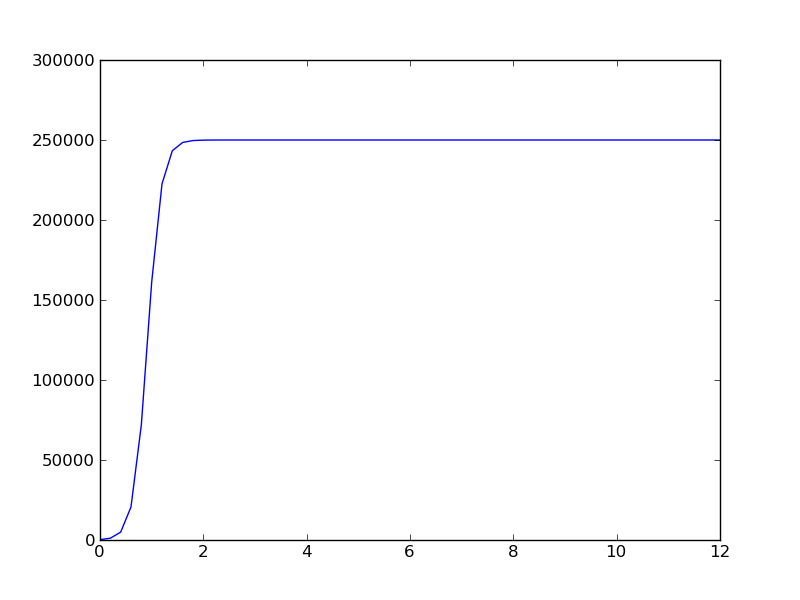
\includegraphics[height=2in, interpolate=true]{data/population_ode}
\end{center}
\end{frame}

% \begin{frame}[fragile]
% \frametitle{ODEs - Simple Pendulum}
% We shall use the simple ODE of a simple pendulum. 
% \begin{equation*}
% \ddot{\theta} = -\frac{g}{L}sin(\theta)
% \end{equation*}
% \begin{itemize}
% \item This equation can be written as a system of two first order ODEs
% \end{itemize}
% \begin{align}
% \dot{\theta} &= \omega \\
% \dot{\omega} &= -\frac{g}{L}sin(\theta) \\
%  \text{At}\ t &= 0 : \nonumber \\
%  \theta = \theta_0(10^o)\quad & \&\quad  \omega = 0\ (Initial\ values)\nonumber 
% \end{align}
% \end{frame}
% 
% \begin{frame}[fragile]
% \frametitle{ODEs - Simple Pendulum \ldots}
% \begin{itemize}
% \item Use \typ{odeint} to do the integration
% \end{itemize}
% \begin{lstlisting}
% In []: def pend_int(initial, t):
%   ....     theta = initial[0]
%   ....     omega = initial[1]
%   ....     g = 9.81
%   ....     L = 0.2
%   ....     F=[omega, -(g/L)*sin(theta)]
%   ....     return F
%   ....
% \end{lstlisting}
% \end{frame}
% 
% \begin{frame}[fragile]
% \frametitle{ODEs - Simple Pendulum \ldots}
% \begin{itemize}
% \item \typ{t} is the time variable \\ 
% \item \typ{initial} has the initial values
% \end{itemize}
% \begin{lstlisting}
% In []: t = linspace(0, 20, 101)
% In []: initial = [10*2*pi/360, 0]
% \end{lstlisting} 
% \end{frame}
% 
% \begin{frame}[fragile]
% \frametitle{ODEs - Simple Pendulum \ldots}
% %%\begin{small}
% \typ{In []: from scipy.integrate import odeint}
% %%\end{small}
% \begin{lstlisting}
% In []: pend_sol = odeint(pend_int, 
%                          initial,t)
% \end{lstlisting}
% \end{frame}
% 
% \begin{frame}[fragile]
% \frametitle{Result}
% \begin{center}
%     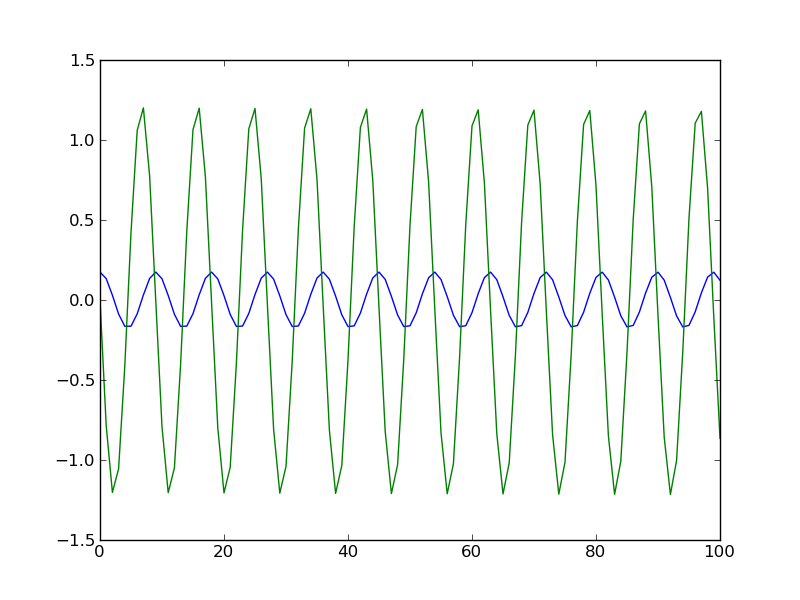
\includegraphics[height=2in, interpolate=true]{data/pendulum_ode}
% \end{center}
%   \inctime{10}
% \end{frame}

\begin{frame}[plain]
    \frametitle{Lorenz equation example}
    \begin{eqnarray*}
        \frac{d x}{dt} &=& s (y-x)\\
        \frac{d y}{d t} &=& rx -y -xz\\
        \frac{d z}{d t} &=& xy - bz\\
    \end{eqnarray*}
    \begin{itemize}
        \item Specifies the evolution of the system
        \item Think: Velocity of a particle in 3D
        \item Lets trace its path
    \end{itemize}
\end{frame}

\begin{frame}[plain,fragile]
    \frametitle{Solution}
\footnotesize
  \begin{lstlisting}
import numpy as np
from scipy.integrate import odeint

def lorenz(r, t s=10.,r=28., b=8./3.):
    x, y, z = r
    u = s*(y-x)
    v = r*x -y - x*z
    w = x*y - b*z
    return np.array([u, v, w])

start = (10., 50., 50.)
t = np.linspace(0., 50., 2000)
r = odeint(lorenz, start, t)
x, y, z = r[:,0], r[:,1], r[:,2]

mlab.plot3d(x, y, z, t, 
from mayavi import mlab
                tube_radius=None)
\end{lstlisting}
\end{frame}

\BackgroundPicture{data/lorenz_traj}
\begin{frame}[plain]
\end{frame}
\BackgroundPicture{data/blank}

\begin{frame}
  \frametitle{Now what?}
  \begin{itemize}
      \item An application to explore these
      \item Use cases
          \begin{itemize}
              \item Interactive exploration
              \item Change the equations on UI
              \item See output immediately
              \item Standard equations (fully setup)
          \end{itemize}
 \end{itemize}
\end{frame}


\begin{frame}
  \frametitle{ETS: Enthought Tool Suite}
  \begin{itemize}
    \item Traits: Object Models
    \item TraitsUI: Views for Traits Objects
    \item Chaco: 2D Visualizations
    \item Mayavi: 3D Visualizations
    \item Envisage: Application Framework
    \vspace*{0.5in}
    \item Miscellaneous libraries
  \end{itemize}
\end{frame}



%%%%%%%%%%%%%%%%%%%%%%%%%%%%%%%%%%%%%%%%%%%%%%%%%%%%%%%%%%%%%%%%%%%%%%%%%%%%%%%
\section{Traits}

\begin{frame}
  \frametitle{Introduction to Traits}
  \begin{itemize}
    \item A \alert{trait} is a type definition that can be used for normal
        Python object attributes giving them additional characteristics.
    \vspace*{2em}

    \item \url{http://code.enthought.com/projects/traits}
    \item \url{http://github.enthought.com/traits/tutorials}

  \end{itemize}
\end{frame}

\begin{frame}
  \frametitle{Trait features}
  \begin{itemize}
    \item Initialization: default value
    \item Validation: strongly typed
    \item Delegation: value delegation
    \item Notification: events
    \item Visualization: MVC, automatic GUI!
  \end{itemize}
\end{frame}

\begin{frame}[fragile,plain]
  \frametitle{Traits Example}
\vspace*{-16pt}
\footnotesize
\begin{lstlisting}
from traits.api import (Delegate, HasTraits, 
    Instance, Int, Str)

class Parent(HasTraits):
    # INITIALIZATION: 'last_name' initialized to ''
    last_name = Str('') 
\end{lstlisting}
\pause
\begin{lstlisting}
class Child(HasTraits):
    age = Int
    # VALIDATION: 'father' must be Parent instance
    father = Instance(Parent)
    # DELEGATION: 'last_name' delegated to father's 
    last_name = Delegate('father') 
    # NOTIFICATION: Method called when 'age' changes
    def _age_changed(self, old, new): 
        print 'Age changed from %s to %s ' % (old, new)
\end{lstlisting}
\end{frame}

\begin{frame}[fragile,plain]
  \frametitle{Traits Example}
\vspace*{-6pt}
\small
\begin{lstlisting}
In []: joe = Parent()
In []: joe.last_name = 'Johnson'
In []: moe = Child()
In []: moe.father = joe

In []: moe.last_name # Delegation
Out[]: "Johnson"

In []: moe.age = 10 # Notification
Age changed from 0 to 10

In []: moe.configure_traits() # Visualization
\end{lstlisting}
\inctime{10}
\end{frame}


\begin{frame}[fragile,plain]
    \frametitle{Predefined Trait Types}
    \vspace*{-6pt}
    \small
    \begin{itemize}
        \item Standard: Bool, Int, Float, Str, Tuple, List, Dict
        \item Constrained: Range, Regex, Expression, ReadOnly
        \item Special: Either, Enum, Array, File, Color, Font
        \item Generic: Instance, Any, Callable
        \item ...
        \item custom traits
    \end{itemize}
\end{frame}

\begin{frame}[fragile,plain]
    \frametitle{Trait Change Notifications}
    \vspace*{-6pt}
    \small
    \begin{itemize}
        \item Static: def \_<trait\_name>\_changed()
        \item Decorator: @on\_trait\_change('extended.trait[].name')
        \item Dynamic: myobject.on\_trait\_change(handler, 'extended.trait[].name')
    \end{itemize}
\end{frame}


\begin{frame}
  \frametitle{Designing the ODE explorer app}
  \Large
\begin{center}
    \myemph{Think!}
\end{center}
\end{frame}

\begin{frame}
  \frametitle{Object model}
  \begin{itemize}
      \item A class to represent the equation and parameters?
      \item A class for the ODE solution
      \item Make sure it works! - TDD
 \end{itemize}
\end{frame}


\begin{frame}[fragile,plain]
    \frametitle{Lorenz Equation}
\scriptsize
\begin{lstlisting}
class LorenzEquation(HasTraits):
    s = Float(10)
    r = Float(28)
    b = Float(8./3)
    
    def eval(self, X, t):
        x, y, z = X[0], X[1], X[2]
        return numpy.array([self.s*(y-x),
                            self.r*x - y - x*z,
                            x*y - self.b*z])
\end{lstlisting}
\end{frame}


\begin{frame}[fragile,plain]
\frametitle{ODE Equation model}
Lets generalize it.
\scriptsize
\begin{lstlisting}
class ODE(HasTraits):
    """ An ODE of the form dX/dt = f(X) """
    name = Str
    num_vars = Int
    vars = Either(List(Str), Str, desc='The names of variables')
    t_var = Str('Time')

    def eval(self, X, t):
        """ Evaluate the derivative function f(X). """
        raise NotImplementedError
\end{lstlisting}
\end{frame}


\begin{frame}[fragile,plain]
\frametitle{Lorenz Equation as an ODE Subclass}
\scriptsize
\begin{lstlisting}
class LorenzEquation(ODE):
    name = 'Lorenz Equation'
    num_vars = 3
    vars = ['x', 'y', 'z']
    s = Float(10)
    r = Float(28)
    b = Float(8./3)

    def eval(self, X, t):
        x, y, z = X[0], X[1], X[2]
        return numpy.array([self.s*(y-x),
                             self.r*x - y - x*z,
                             x*y - self.b*z])
\end{lstlisting}
\end{frame}


\begin{frame}[fragile,plain]
\frametitle{ODESolver}
Someone needs to solve the ODE!
\scriptsize
\begin{lstlisting}
class ODESolver(HasTraits):
    """ A solver for the ODE (fixed initial condn.) """
    ode = Instance(ODE)
    initial_state = Either(Float, Array)
    t_arr = Array
    soln_arr = Property(Array, depends_on='initial_state, t_arr, ode')

    @cached_property
    def _get_soln_arr(self):
        return self.solve()

    def solve(self):
        """ Solve the ODE and return the values of the solution vector at
        specified times t. """
        return odeint(self.ode.eval, self.initial_state, self.t_arr)
\end{lstlisting}
\end{frame}

\begin{frame}[fragile,plain]
\frametitle{Testing}
Does it work?
\scriptsize
\begin{lstlisting}
class TestLorenzEquation(unittest.TestCase):
    def setUp(self):
        self.ode = LorenzEquation()
        self.solver = ODESolver(ode=self.ode, initial_state=[10.,50.,50.], t_arr=numpy.linspace(0,10,1001))

    def test_eval(self):
        dX = self.ode.eval(self.solver.initial_state, 0.0)
        self.assertAlmostEqual(dX[0], 400)
        self.assertAlmostEqual(dX[1], -270)
        self.assertAlmostEqual(dX[2], 1100/3.)

    def test_solve(self):
        soln = self.solver.soln_arr[1,:]
        self.assertAlmostEqual(soln[0], 13.65484958)
        self.assertAlmostEqual(soln[1], 46.64090341)
        self.assertAlmostEqual(soln[2], 54.35797299)
\end{lstlisting}
\end{frame}




%%%%%%%%%%%%%%%%%%%%%%%%%%%%%%%%%%%%%%%%%%%%%%%%%%%%%%%%%%%%%%%%%%%%%%%%%%%%%%%
\section{TraitsUI}

\begin{frame}
  \frametitle{TraitsUI}
  \begin{itemize}
      \item Implement MVC design pattern
      \item Create default views for models
      \item Keep multiple views synced with model
      \item Create UI with minimal toolkit knowledge
  \end{itemize}
\end{frame}

\begin{frame}[fragile,plain]
\frametitle{Default Traits View}
\begin{lstlisting}
father = Parent(last_name='Joe')
child = Child(age=2, father=father)
child.configure_traits()
\end{lstlisting}
\pause
\begin{itemize}
\item Automatic UI creation with \emph{configure\_traits()}
\item Automatic sync with model
\item Automatic sync between different views
\end{itemize}
\end{frame}

\begin{frame}[fragile,plain]
\frametitle{Lorenz Equation View}
Configure the parameters of the Lorenz equation \emph{s}, \emph{r} and \emph{b}
\scriptsize
\begin{lstlisting}
class LorenzEquation(ODE):
    ...
    view = View(Item('s', editor=RangeEditor(low=0.0, high=20.0)),
                Item('r', editor=RangeEditor(low=20.0, high=36.0)),
                Item('b', editor=RangeEditor(low=0.0, high=5.0)))
\end{lstlisting}
\end{frame}



%%%%%%%%%%%%%%%%%%%%%%%%%%%%%%%%%%%%%%%%%%%%%%%%%%%%%%%%%%%%%%%%%%%%%%%%%%%%%%%
\section{Chaco}

\begin{frame}
  \frametitle{Chaco}
  \begin{itemize}
      \item XXX
 \end{itemize}
\end{frame}

%%%%%%%%%%%%%%%%%%%%%%%%%%%%%%%%%%%%%%%%%%%%%%%%%%%%%%%%%%%%%%%%%%%%%%%%%%%%%%%
\section{Mayavi}

\begin{frame}
  \frametitle{Mayavi}
  \begin{itemize}
      \item XXX
 \end{itemize}
\end{frame}

%%%%%%%%%%%%%%%%%%%%%%%%%%%%%%%%%%%%%%%%%%%%%%%%%%%%%%%%%%%%%%%%%%%%%%%%%%%%%%%
\section{Putting all together}

\begin{frame}
  \frametitle{The application}
  \begin{itemize}
      \item XXX
 \end{itemize}
\end{frame}

%%%%%%%%%%%%%%%%%%%%%%%%%%%%%%%%%%%%%%%%%%%%%%%%%%%%%%%%%%%%%%%%%%%%%%%%%%%%%%%
\section{Note on Envisage}

\begin{frame}
  \frametitle{Envisage}
  \begin{itemize}
      \item XXX
 \end{itemize}
\end{frame}

\section{Summary}

\begin{frame}
  \frametitle{Summary}
  \begin{itemize}
      \item XXX
 \end{itemize}
\end{frame}

\end{document}

%%%%%%%%%%%%%%%%%%%%%%%%%%%%%%%%%%%%%%%%%%%%%%%%%%%%%%%%%%%%%%%%%%%%%%%%%%%%%%%



